\documentclass[10pt]{article}

\usepackage[utf8]{inputenc}
\usepackage[a4paper,total={6.2in,9.0in}]{geometry}

\usepackage{
graphicx,
amsmath,
amssymb,
booktabs,
float,
fancyhdr,
titlesec,
cite,
hyperref,
xcolor,
tikz,
array
}

\usetikzlibrary{
positioning,
arrows.meta,
shapes.geometric,
calc
}

\hypersetup{hidelinks}

%---------------- Page layout ----------------

\setlength{\parindent}{0pt}
\setlength{\parskip}{2.5pt}
\setlength{\textfloatsep}{6pt}
\setlength{\floatsep}{5pt}
\setlength{\intextsep}{5pt}
\emergencystretch=2em

%---------------- Header ----------------

\pagestyle{fancy}
\fancyhf{}
\lhead{230449N}
\rhead{PPG Signal Acquisition and Conditioning}
\cfoot{\thepage}

%---------------- Section formatting ----------------

\titleformat{\section}
{\large\bfseries}
{\thesection}
{0.7em}
{}

\titleformat{\subsection}
{\normalsize\bfseries}
{\thesubsection}
{0.5em}
{}

\titlespacing*{\section}{0pt}{5pt}{2pt}
\titlespacing*{\subsection}{0pt}{3pt}{1pt}

%---------------- TikZ styles ----------------

\tikzset{
box/.style={
draw,
rounded corners=2pt,
thick,
align=center,
minimum height=.65cm,
minimum width=1.65cm,
fill=gray!10
},
smallbox/.style={
draw,
rounded corners=2pt,
align=center,
minimum height=.5cm,
minimum width=1.25cm,
fill=gray!7
},
arrow/.style={
-{Latex[length=1.7mm]},
thick
}
}

%================ DOCUMENT =================

\begin{document}

%================================================
% TITLE PAGE
%================================================

\begin{titlepage}

\centering

\IfFileExists{campus_logo.png}
{

\includegraphics[width=3.5cm]{campus_logo.png}
}
{
\fbox{
\parbox[c][3.5cm][c]{3.5cm}
{\centering University of Moratuwa}
}
}

\vspace{0.35cm}

{\large
Department of Electronic \& Telecommunication Engineering\\
University of Moratuwa
}

\vspace{1.4cm}

{\Huge\bfseries
Photoplethysmography\\
(PPG) Signal Acquisition and Conditioning
}

\vspace{0.5cm}

{\Large
Design, Simulation and Analysis of a PPG Circuit
}

\vfill

\begin{tabular}{ll}
Name: & W.A.S. Nuwanaka\\
Index: & 230449N\\
Semester: & 05\\
Course: & BM3110/EN3533 Electronic Instrumentation
\end{tabular}

\vfill

\today

\end{titlepage}

%================================================
% CONTENTS
%================================================

\tableofcontents
\newpage

%================================================
% 1. INTRODUCTION
%================================================

\section{Introduction}

\subsection{Background}

Photoplethysmography (PPG) is a non-invasive optical technique used to detect variations in blood volume within biological tissue. A typical PPG system consists of a light source, usually an LED, and a photodetector such as a photodiode. The light is transmitted into or reflected from the tissue, and the changes in the detected optical intensity are converted into an electrical signal.

The PPG signal contains a small pulsatile component associated with changes in arterial blood volume caused by the cardiac cycle. It is generally superimposed on a much larger slowly varying DC component caused by tissue, venous blood, average blood volume and the optical properties of the measurement site. Consequently, signal conditioning is required before the PPG signal can be reliably observed or processed.

PPG signals are widely used in biomedical instrumentation. Applications include heart-rate monitoring, pulse oximetry, vascular assessment and wearable health-monitoring devices. The simplicity of optical sensing makes PPG particularly suitable for portable and low-cost medical and consumer devices.

\begin{figure}[H]
\centering
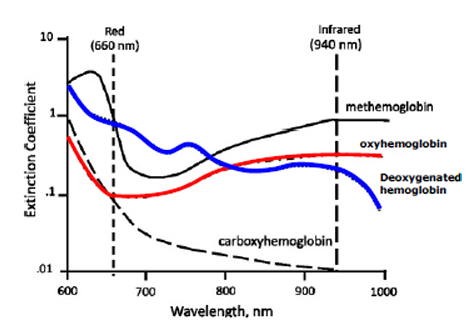
\includegraphics[width=0.45\textwidth]{absorbance_spectrum.png}
\caption{Absorbance spectrum of transmitted light of haemoglobin. The red line indicates the extinction strength of oxygenated haemoglobin; the blue line indicates deoxygenated haemoglobin \cite{james}.}
\end{figure}

\subsection{Importance of PPG}

The main advantage of PPG is that it allows cardiovascular information to be obtained without an invasive procedure. The periodicity of the pulsatile waveform can be used to estimate heart rate, while the waveform morphology contains information related to blood flow and vascular behaviour.

However, the amplitude of the AC component of a PPG signal is relatively small compared with the DC component. Furthermore, the signal can be affected by ambient light, motion artefacts, power-line interference and electronic noise. Therefore, amplification and filtering are essential parts of a practical PPG instrumentation system.

\begin{figure}[H]
\centering
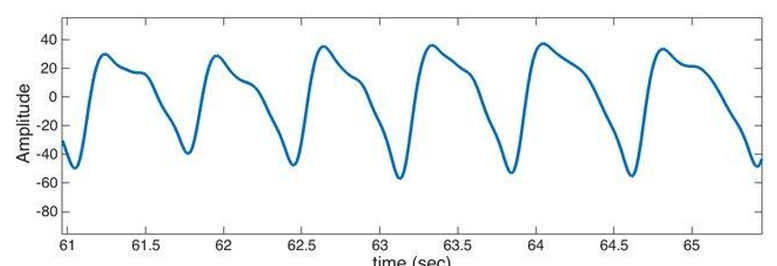
\includegraphics[width=0.65\textwidth]{../Typical plethysmographic waveform as seen on a plethysmogram for clinical use.png}
\caption{Typical plethysmographic waveform as seen on a plethysmogram for clinical use \cite{james}.}
\end{figure}

\subsection{Objectives}

The main objectives of this practical are:

\begin{itemize}
    \item To understand the operating principle of a photoplethysmography system.
    \item To design a circuit capable of detecting the optical variation associated with blood-volume changes.
    \item To amplify the small electrical signal produced by the photodetector.
    \item To design suitable high-pass and low-pass filtering stages.
    \item To reduce unwanted low-frequency drift and high-frequency noise.
    \item To simulate the circuit using LTspice.
    \item To observe and analyse the waveform at different stages of the circuit.
    \item To determine the amplitude and duration of the final PPG waveform.
    \item To implement a PI controller for automatic LED current regulation.
    \item To consider practical implementation issues when transferring the circuit to a PCB.
\end{itemize}

%================================================
% 2. MATERIALS AND METHODS
%================================================

\section{Materials and Methods}

\subsection{Equipment and Components}

The following components and equipment were used for the design and simulation of the PPG circuit:

\begin{table}[H]
\centering
\caption{Main components used in the PPG signal-conditioning circuit.}
\begin{tabular}{lll}
\toprule
Component & Typical value/type & Purpose\\
\midrule
LED & NSCW100 (White LED) & Optical illumination\\
MOSFET & BSS123 (N-channel) & LED current switching\\
Operational amplifier & TS912 (rail-to-rail) & Signal amplification / filtering\\
Resistors & Various (10\,$\Omega$ -- 1\,M$\Omega$) & Gain, bias and filter design\\
Capacitors & 470\,nF -- 10\,$\mu$F & AC coupling and filtering\\
DC supply & $+5$\,V / $+2.5$\,V / GND & Circuit power supply\\
LTspice & Simulation software & Circuit simulation\\
\bottomrule
\end{tabular}
\end{table}

\subsection{Reason for Using Each Component}

\subsubsection{LED (NSCW100)}

The NSCW100 white LED provides optical illumination to the measurement site. When blood volume changes during the cardiac cycle, the amount of light absorbed or reflected by the tissue changes. This produces a corresponding variation in the light received by the photodetector.

\subsubsection{MOSFET (BSS123)}

The BSS123 N-channel MOSFET acts as a voltage-controlled current switch for driving the LED. The gate voltage, controlled by the op-amp output through a series resistor, regulates the drain current flowing through the LED. This arrangement enables precise control of the LED drive current.

\subsubsection{Operational Amplifier (TS912)}

The TS912 is a dual rail-to-rail input/output CMOS operational amplifier. It is used in several configurations throughout the circuit:
\begin{itemize}
    \item As a voltage follower / buffer in the emitter driver stage.
    \item As a transimpedance amplifier (TIA) for converting photodiode current to voltage.
    \item As a non-inverting amplifier for signal gain.
    \item As active filter stages (integrator / band-pass).
    \item In the PI controller for automatic LED current regulation.
\end{itemize}

\subsubsection{Resistors}

Resistors determine amplifier gain, establish bias conditions, form the resistive components of the filter networks and set the LED drive current through the sense resistor.

\subsubsection{Capacitors}

Capacitors are used for AC coupling and frequency-selective filtering. In particular, a capacitor in combination with a resistor can be used to form a high-pass filter that attenuates the DC component and slow baseline variations, or a low-pass filter to attenuate high-frequency noise.

\subsection{Stages of the PPG Circuit}

The complete PPG signal-conditioning system can be divided into several functional stages. The overall system block diagram is shown below.

\begin{figure}[H]
\centering
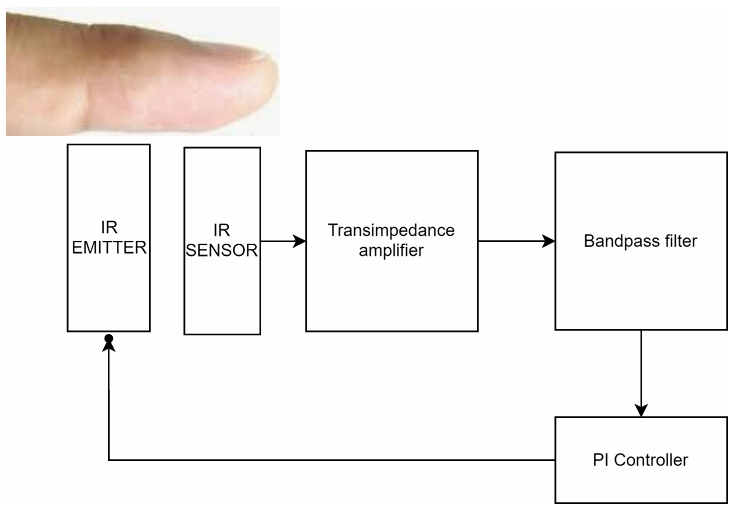
\includegraphics[width=0.55\textwidth]{../Basic block diagram.png}
\caption{Overall block diagram of the PPG system showing the IR emitter, IR sensor, transimpedance amplifier, bandpass filter and PI controller feedback loop.}
\end{figure}

\begin{figure}[H]
\centering
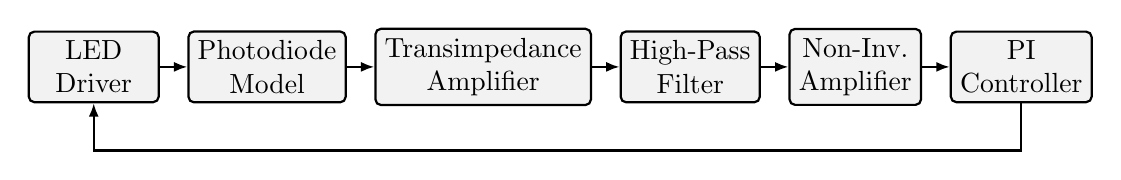
\begin{tikzpicture}[node distance=0.35cm]
\node[box] (led) {LED\\Driver};
\node[box, right=of led] (pd) {Photodiode\\Model};
\node[box, right=of pd] (tia) {Transimpedance\\Amplifier};
\node[box, right=of tia] (hp) {High-Pass\\Filter};
\node[box, right=of hp] (amp) {Non-Inv.\\Amplifier};
\node[box, right=of amp] (pi) {PI\\Controller};

\draw[arrow] (led) -- (pd);
\draw[arrow] (pd) -- (tia);
\draw[arrow] (tia) -- (hp);
\draw[arrow] (hp) -- (amp);
\draw[arrow] (amp) -- (pi);
\draw[arrow] (pi.south) -- ++(0,-0.6) -| (led.south);
\end{tikzpicture}
\caption{Functional block diagram of the PPG signal-conditioning system with PI controller feedback.}
\end{figure}

The main stages are:

\begin{enumerate}
    \item Optical excitation using an LED driven by a MOSFET current source.
    \item Simulation of the photodiode response using current sources (DC pulse, AC cardiac pulse and 100\,Hz noise).
    \item Conversion of the photodiode current into a voltage using a transimpedance amplifier.
    \item High-pass filtering to suppress the DC component and baseline drift.
    \item Amplification of the small pulsatile signal using a non-inverting amplifier.
    \item PI controller feedback to regulate the LED drive current and maintain a stable operating point.
    \item Observation of the conditioned PPG waveform.
\end{enumerate}

\subsection{Step-by-Step Development}

The circuit was developed incrementally in four stages within a single LTspice schematic:

\textbf{Stage 1 -- The Emitter:} The LED driver circuit was designed first. A TS912 op-amp buffers a PULSE voltage source (100\,mV to 400\,mV, period 1\,s) and drives the gate of a BSS123 MOSFET through a 1\,k$\Omega$ series resistor (R5). The MOSFET switches current through the NSCW100 LED from a 5\,V supply. A 10\,$\Omega$ sense resistor (R6) allows measurement of the LED current.

\textbf{Stage 2 -- The Receiver:} The receiver was designed independently using three current sources to model the photodiode output:
\begin{itemize}
    \item I1: PULSE(0, 30\,$\mu$A, 1\,s delay, 5\,s on, 10\,s period) -- models the DC component.
    \item I2: SINE(0, 10\,$\mu$A, 100\,Hz) -- models ambient noise / interference.
    \item I3: PULSE(0, 10\,$\mu$A, 0, 1\,$\mu$s, 1\,$\mu$s, 100\,ms, 1\,s) -- models the cardiac pulse.
\end{itemize}
The current is fed into a TS912 transimpedance amplifier (U1) with a 10\,k$\Omega$ feedback resistor (R1) and 1\,$\mu$F feedback capacitor (C2), forming a low-pass characteristic. The output is AC-coupled through a 10\,$\mu$F capacitor (C1) to a non-inverting amplifier (U2) with a gain of $1 + R_2/R_3 = 1 + 10\mathrm{k}/1\mathrm{k} = 11$. A 1\,M$\Omega$ DC bias resistor (R4) and 2.5\,V bias supply (V1, V3) set the operating point.

\textbf{Stage 3 -- Integration of Emitter with Sensor:} The emitter and receiver were combined. The LED driver uses R7 = 90\,k$\Omega$ and R8 = 10\,k$\Omega$ as a voltage divider at the input. The receiver section uses a TIA (U4) with R9 = 1\,k$\Omega$, R10 = 10\,$\Omega$, followed by a second amplifier (U6) with a feedback network of C4 = 1\,$\mu$F and R14 = 10\,k$\Omega$ (forming a low-pass filter), and a coupling capacitor C3 = 1\,$\mu$F. The non-inverting gain stage uses R13 = 70\,k$\Omega$ and R12 = 10\,k$\Omega$, giving a gain of $1 + 70\mathrm{k}/10\mathrm{k} = 8$.

\textbf{Stage 4 -- PPG Sensor with PI Controller:} A proportional-integral (PI) controller was added to regulate the LED drive current automatically. The P-controller uses a summing amplifier (U11) with R28 = R29 = R30 = 1\,M$\Omega$ and R31 = 470\,k$\Omega$ (gain $= -470\mathrm{k}/1\mathrm{M} = -0.47$). The I-controller uses an integrator (U12) with R32 = 1\,M$\Omega$ and C9 = 470\,nF. The PI output feeds back through R25 = 1\,M$\Omega$ and C7 = 1\,$\mu$F to the final non-inverting amplifier (U10) with R27 = 10\,k$\Omega$ and R26 = 1\,k$\Omega$ (gain $= 1 + 10\mathrm{k}/1\mathrm{k} = 11$) and output capacitor C8 = 1\,$\mu$F.

The simulation command used was: \texttt{.tran 0 1s 0 100m}.

%================================================
% 3. CIRCUIT DIAGRAMS
%================================================

\section{Circuit Diagrams}

\subsection{Overall Circuit}

The complete PPG circuit consists of four sections implemented in a single LTspice schematic: The Emitter, The Receiver, Integration of Emitter with Sensor, and PPG Sensor with PI Controller.

\begin{figure}[H]
\centering
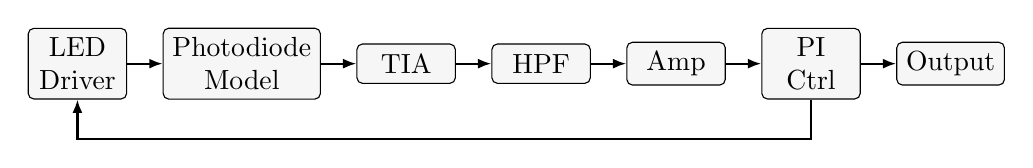
\begin{tikzpicture}[node distance=0.55cm and 0.45cm]

\node[smallbox] (led) {LED\\Driver};
\node[smallbox, right=of led] (sensor) {Photodiode\\Model};
\node[smallbox, right=of sensor] (tia) {TIA};
\node[smallbox, right=of tia] (hp) {HPF};
\node[smallbox, right=of hp] (amp) {Amp};
\node[smallbox, right=of amp] (pi) {PI\\Ctrl};
\node[smallbox, right=of pi] (out) {Output};

\draw[arrow] (led) -- (sensor);
\draw[arrow] (sensor) -- (tia);
\draw[arrow] (tia) -- (hp);
\draw[arrow] (hp) -- (amp);
\draw[arrow] (amp) -- (pi);
\draw[arrow] (pi) -- (out);
\draw[arrow] (pi.south) -- ++(0,-0.5) -| (led.south);

\end{tikzpicture}
\caption{Simplified schematic representation of the PPG system with PI feedback.}
\end{figure}

\subsection{Emitter Stage}

The emitter circuit drives the NSCW100 LED using a BSS123 N-channel MOSFET. The op-amp (TS912) acts as a voltage follower, buffering the input signal and driving the MOSFET gate through a 1\,k$\Omega$ resistor. The 10\,$\Omega$ sense resistor allows monitoring of the LED current.

\begin{figure}[H]
\centering
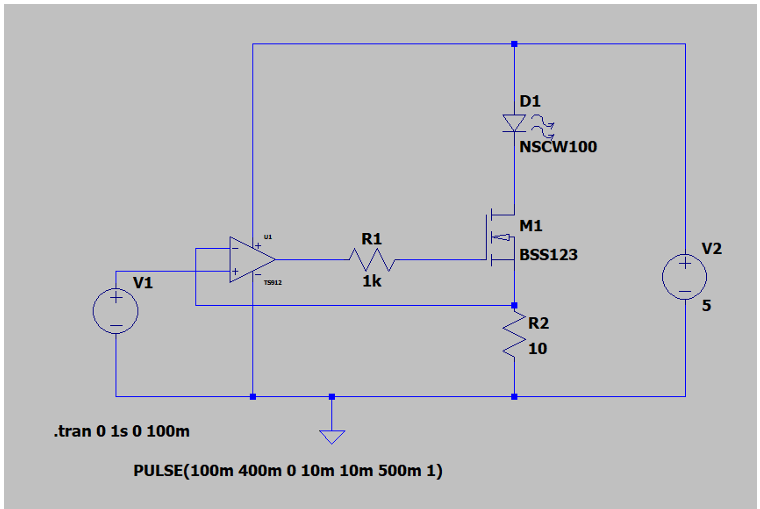
\includegraphics[width=0.55\textwidth]{../Design of the sensor/The picture of Emitter.png}
\caption{LTspice schematic of the LED emitter driver circuit. V1 provides the PULSE input (100--400\,mV), U1 (TS912) buffers the signal, M1 (BSS123) switches the LED current, and D1 (NSCW100) is the LED.}
\end{figure}

\subsection{Receiver Stage (Transimpedance Amplifier and Non-Inverting Amplifier)}

The photodiode is modelled by three parallel current sources. The transimpedance amplifier converts the photodiode current into a voltage. The output is AC-coupled and further amplified by a non-inverting amplifier with a gain of 11.

For the transimpedance amplifier, the approximate output voltage is

\begin{equation}
V_{\mathrm{out}}=-I_{\mathrm{PD}} \cdot R_f = -I_{\mathrm{PD}} \times 10\,\mathrm{k\Omega}.
\end{equation}

The feedback capacitor $C_2 = 1\,\mu$F limits the bandwidth and improves stability. The $-3$\,dB frequency of the TIA is

\begin{equation}
f_{-3\mathrm{dB}} = \frac{1}{2\pi R_f C_f} = \frac{1}{2\pi (10\times10^3)(1\times10^{-6})} \approx 15.9\,\mathrm{Hz}.
\end{equation}

\begin{figure}[H]
\centering
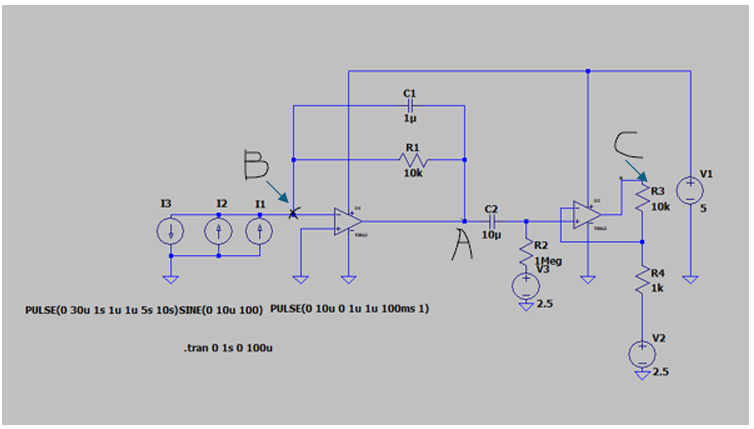
\includegraphics[width=0.75\textwidth]{../Design of the sensor/The LTC Spice model of the receiver.png}
\caption{LTspice schematic of the receiver. Three current sources (I1, I2, I3) model the photodiode. Op-amp A is the TIA with R1 = 10\,k$\Omega$ and C1 = 1\,$\mu$F. C2 = 10\,$\mu$F provides AC coupling. Op-amp C is the non-inverting amplifier with R3 = 10\,k$\Omega$ and R4 = 1\,k$\Omega$ (gain = 11). The 2.5\,V sources (V1, V2) set the DC bias.}
\end{figure}

\subsection{High-Pass Filter}

The AC coupling capacitor $C_1 = 10\,\mu$F in series with the 1\,M$\Omega$ bias resistor $R_4$ forms a first-order high-pass filter with cutoff frequency:

\begin{equation}
f_L=\frac{1}{2\pi R C} = \frac{1}{2\pi(1\times10^6)(10\times10^{-6})} \approx 0.016\,\mathrm{Hz}.
\end{equation}

This very low cutoff frequency allows the normal pulsatile component of the PPG signal (typically 0.5--5\,Hz) to pass while attenuating very slow baseline variations and the DC component.

\subsection{Low-Pass Filter}

The TIA feedback network ($R_1 = 10\,\mathrm{k\Omega}$, $C_2 = 1\,\mu$F for the standalone receiver; $R_{14} = 10\,\mathrm{k\Omega}$, $C_4 = 1\,\mu$F for the integrated version) forms a low-pass filter:

\begin{equation}
f_H=\frac{1}{2\pi R C} = \frac{1}{2\pi(10\times10^3)(1\times10^{-6})} \approx 15.9\,\mathrm{Hz}.
\end{equation}

This cutoff frequency is sufficiently high to preserve the PPG waveform harmonics while attenuating the 100\,Hz noise component modelled by current source I2.

\subsection{PI Controller}

A proportional-integral controller was added to automatically regulate the LED brightness, compensating for slow variations in the DC level.

\begin{figure}[H]
\centering
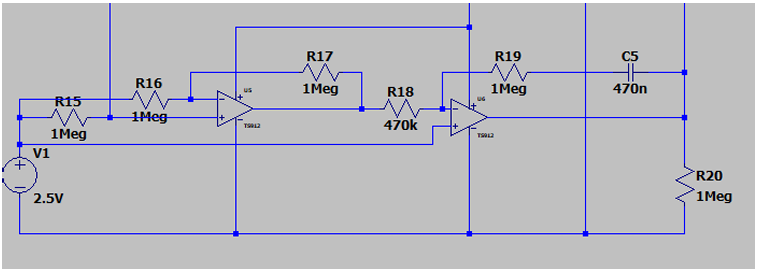
\includegraphics[width=0.75\textwidth]{../Design of the sensor/The PI Controller.png}
\caption{LTspice schematic of the PI controller. The P-controller (U11) uses R15 = R16 = 1\,M$\Omega$ input resistors, R17 = 1\,M$\Omega$ and R18 = 470\,k$\Omega$ feedback. The I-controller (U12) uses R19 = 1\,M$\Omega$ input and C5 = 470\,nF feedback capacitor. R20 = 1\,M$\Omega$ provides a DC bias path.}
\end{figure}

The proportional gain is:
\begin{equation}
K_P = -\frac{R_{18}}{R_{17}} = -\frac{470\,\mathrm{k}}{1\,\mathrm{M}} = -0.47.
\end{equation}

The integrator transfer function is:
\begin{equation}
H_I(s) = -\frac{1}{s R_{19} C_5} = -\frac{1}{s \cdot (1\times10^6)(470\times10^{-9})} = -\frac{1}{0.47\,s}.
\end{equation}

The integrator time constant is $\tau_I = R_{19} C_5 = 0.47\,$s, providing slow correction of the DC operating point.

\subsection{Final Circuit Diagram}

The finalized LTspice schematic contains all four circuit sections on a single sheet.

\begin{figure}[H]
\centering
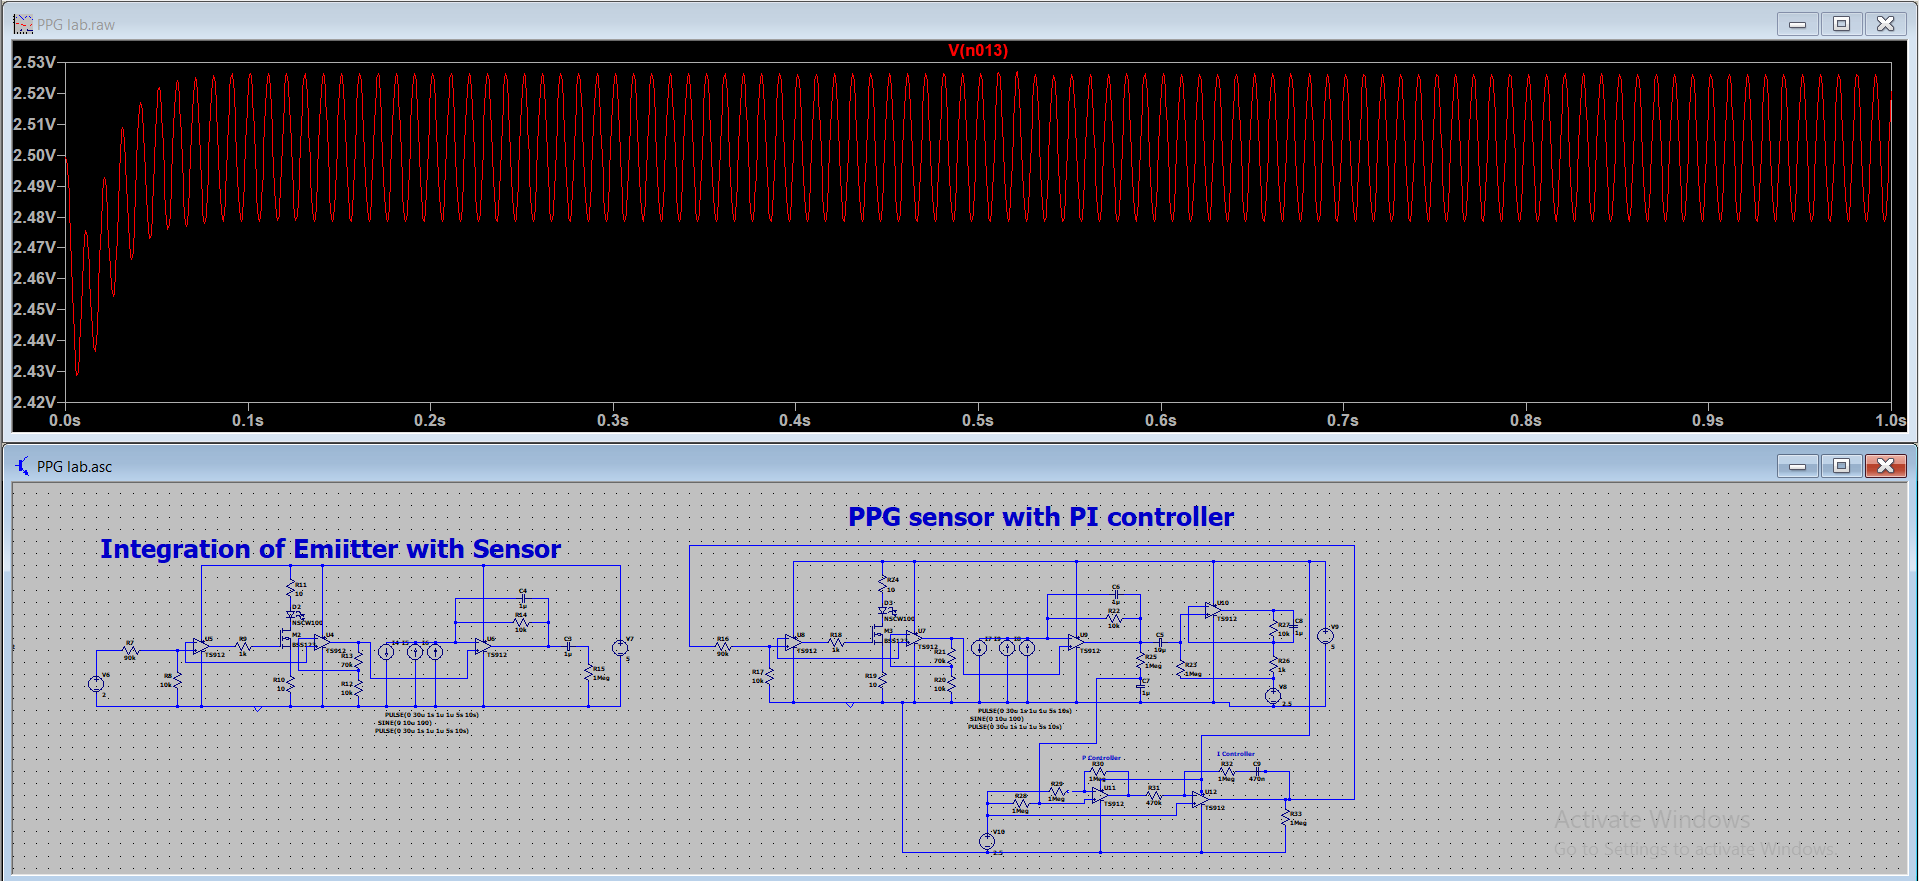
\includegraphics[width=0.95\textwidth]{../With PI controller/Output.png}
\caption{Screenshot of the complete LTspice schematic showing the PPG sensor with PI controller and its output waveform V(n013).}
\end{figure}

%================================================
% 4. OBSERVATIONS
%================================================

\section{Observations}

\subsection{Emitter Stage Waveform}

The emitter stage drives the LED with a controlled current. The gate voltage follows the PULSE input signal, and the LED current switches accordingly. The LED current reaches approximately 40\,mA when the gate voltage is high (corresponding to 400\,mV input) and drops to approximately 12\,mA at the low level.

\begin{figure}[H]
\centering
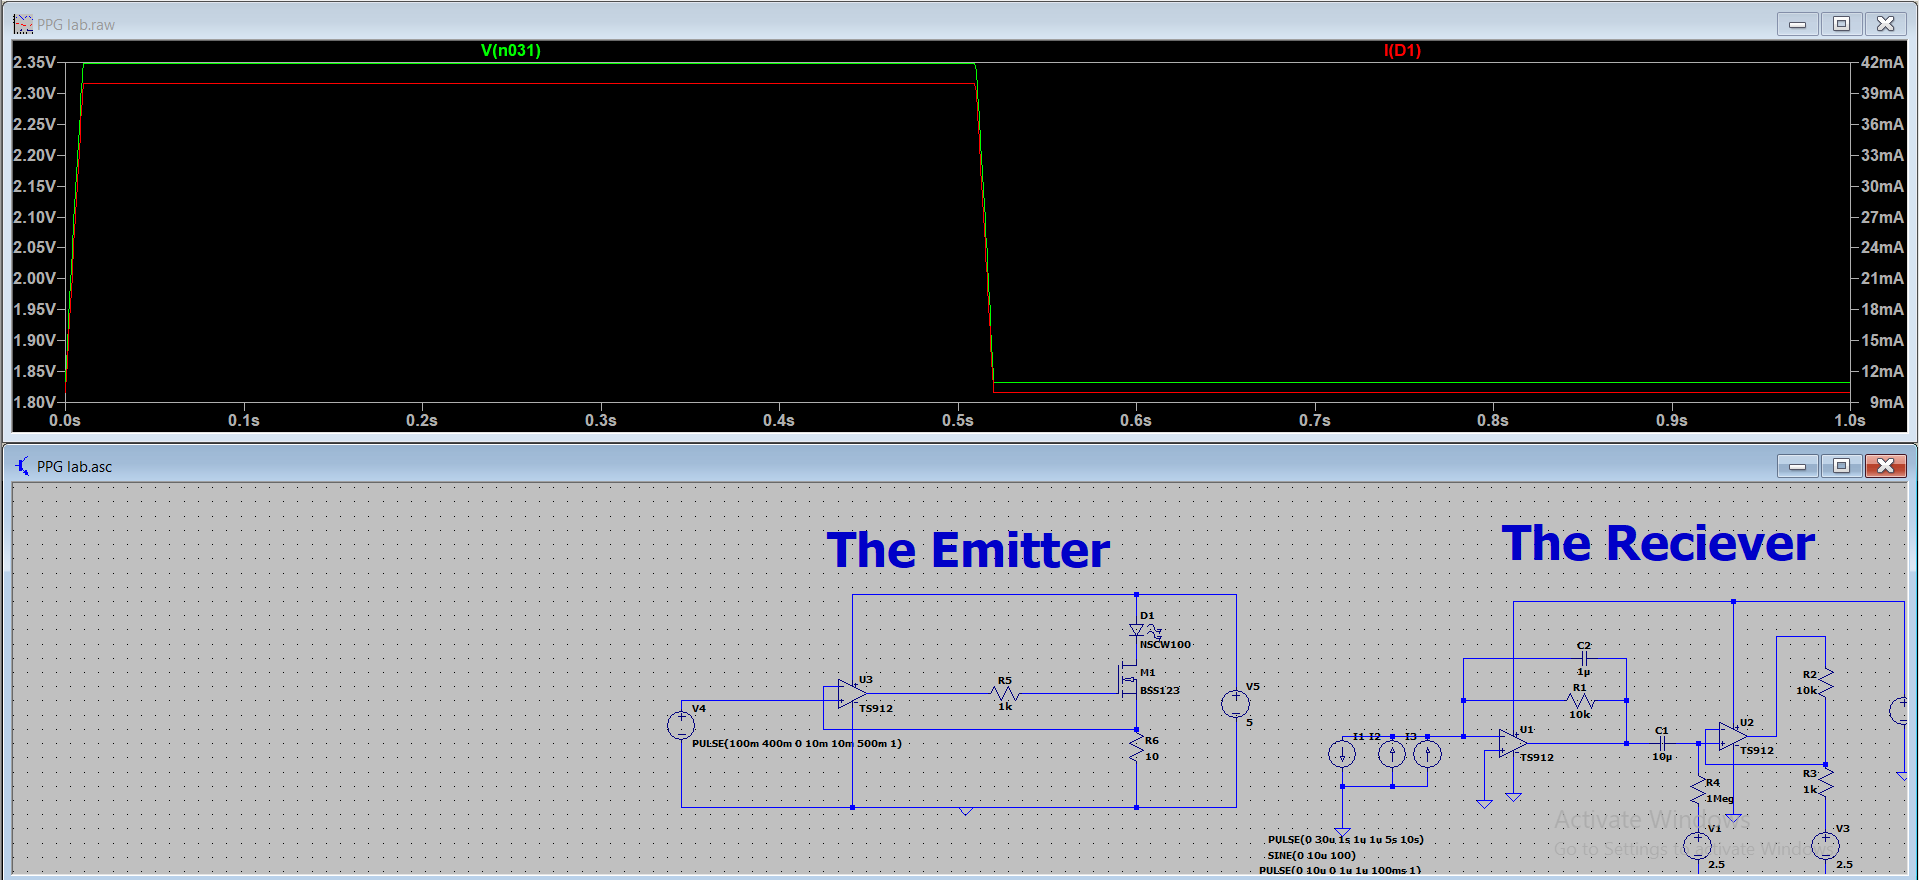
\includegraphics[width=0.82\textwidth]{../Emitter/Emitter MosFET in G LED current R.png}
\caption{Emitter stage waveforms: V(n031) shows the MOSFET gate voltage (green, left axis, 1.80--2.35\,V), and I(D1) shows the LED current (red, right axis, 9--42\,mA). The LED is on for 500\,ms and off for 500\,ms.}
\end{figure}

\subsection{Transimpedance Amplifier Output (Current Adder)}

The TIA converts the combined photodiode current into a voltage. The output shows the DC component due to I1, the pulsatile component from I3, and the 100\,Hz noise from I2 superimposed.

\begin{figure}[H]
\centering
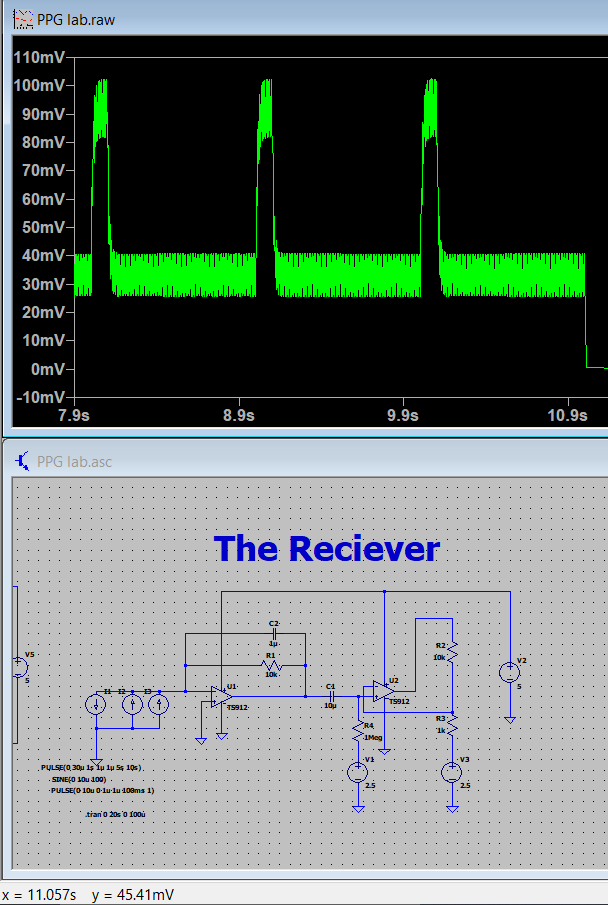
\includegraphics[width=0.82\textwidth]{../Reciever/Current Adder.png}
\caption{Output waveform V(n018) of the current adder / TIA stage. The signal ranges from approximately 24\,mV to 104\,mV, with an initial transient settling within 0.2\,s. The 100\,Hz noise component is clearly visible.}
\end{figure}

\subsection{Non-Inverting Amplifier Output}

After AC coupling and amplification by the non-inverting amplifier (gain = 11), the signal is centred around the 2.5\,V bias and the pulsatile component becomes more prominent.

\begin{figure}[H]
\centering
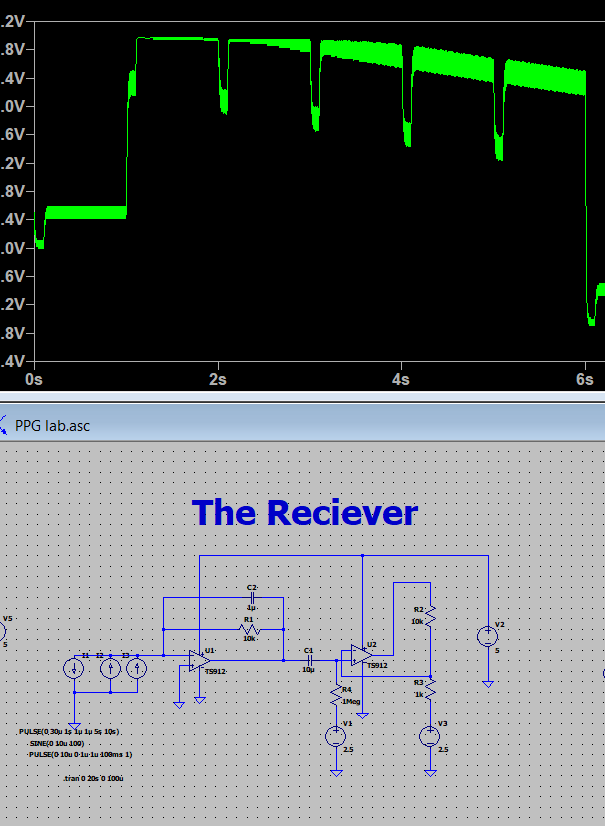
\includegraphics[width=0.82\textwidth]{../Reciever/Non Inverting Amplifier utput.png}
\caption{Output waveform V(n014) of the non-inverting amplifier stage. The signal oscillates between approximately 2.40\,V and 2.60\,V, centred around the 2.5\,V bias. The waveform settles after the initial transient.}
\end{figure}

\subsection{Receiver Integrator / Filter Output}

The integrator stage provides additional low-pass filtering to suppress high-frequency noise.

\begin{figure}[H]
\centering
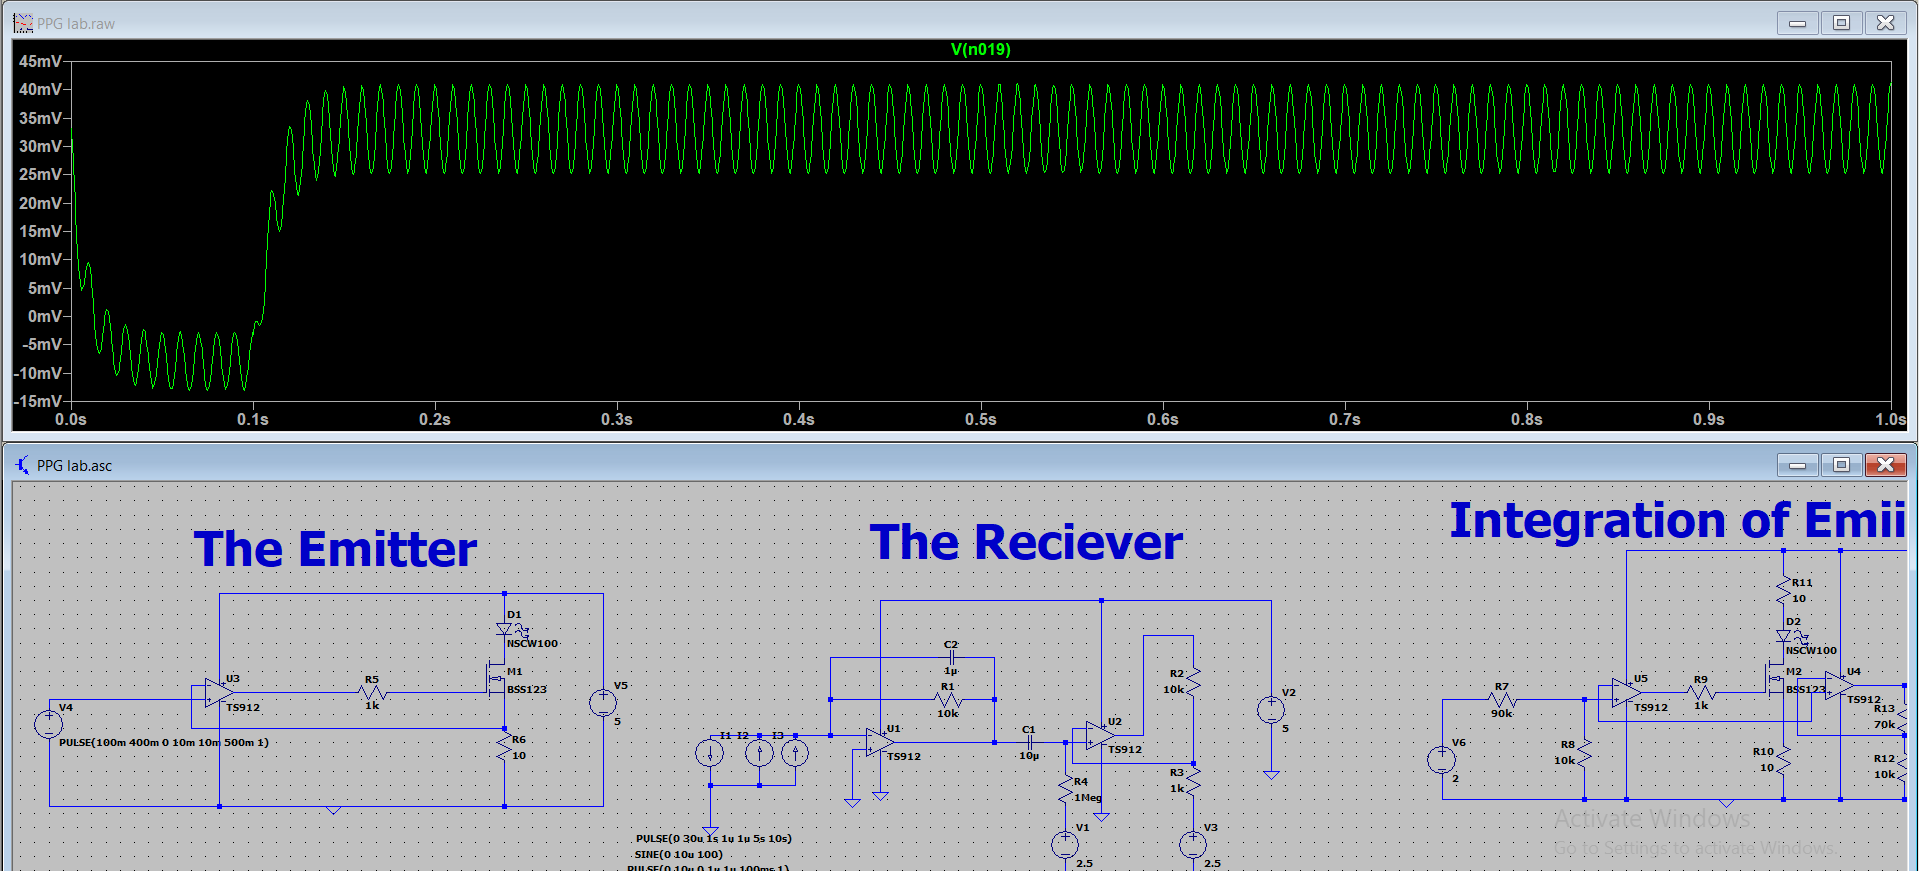
\includegraphics[width=0.82\textwidth]{../Reciever/Reciver Integrater out.png}
\caption{Output waveform V(n019) of the receiver integrator stage. The signal ranges from approximately $-15$\,mV to 45\,mV. The initial transient settles by approximately 0.2\,s.}
\end{figure}

\subsection{Integrated Emitter with Sensor Output}

When the emitter and sensor are combined, the output waveform shows the processed PPG-like signal with both the pulsatile component and residual noise.

\begin{figure}[H]
\centering
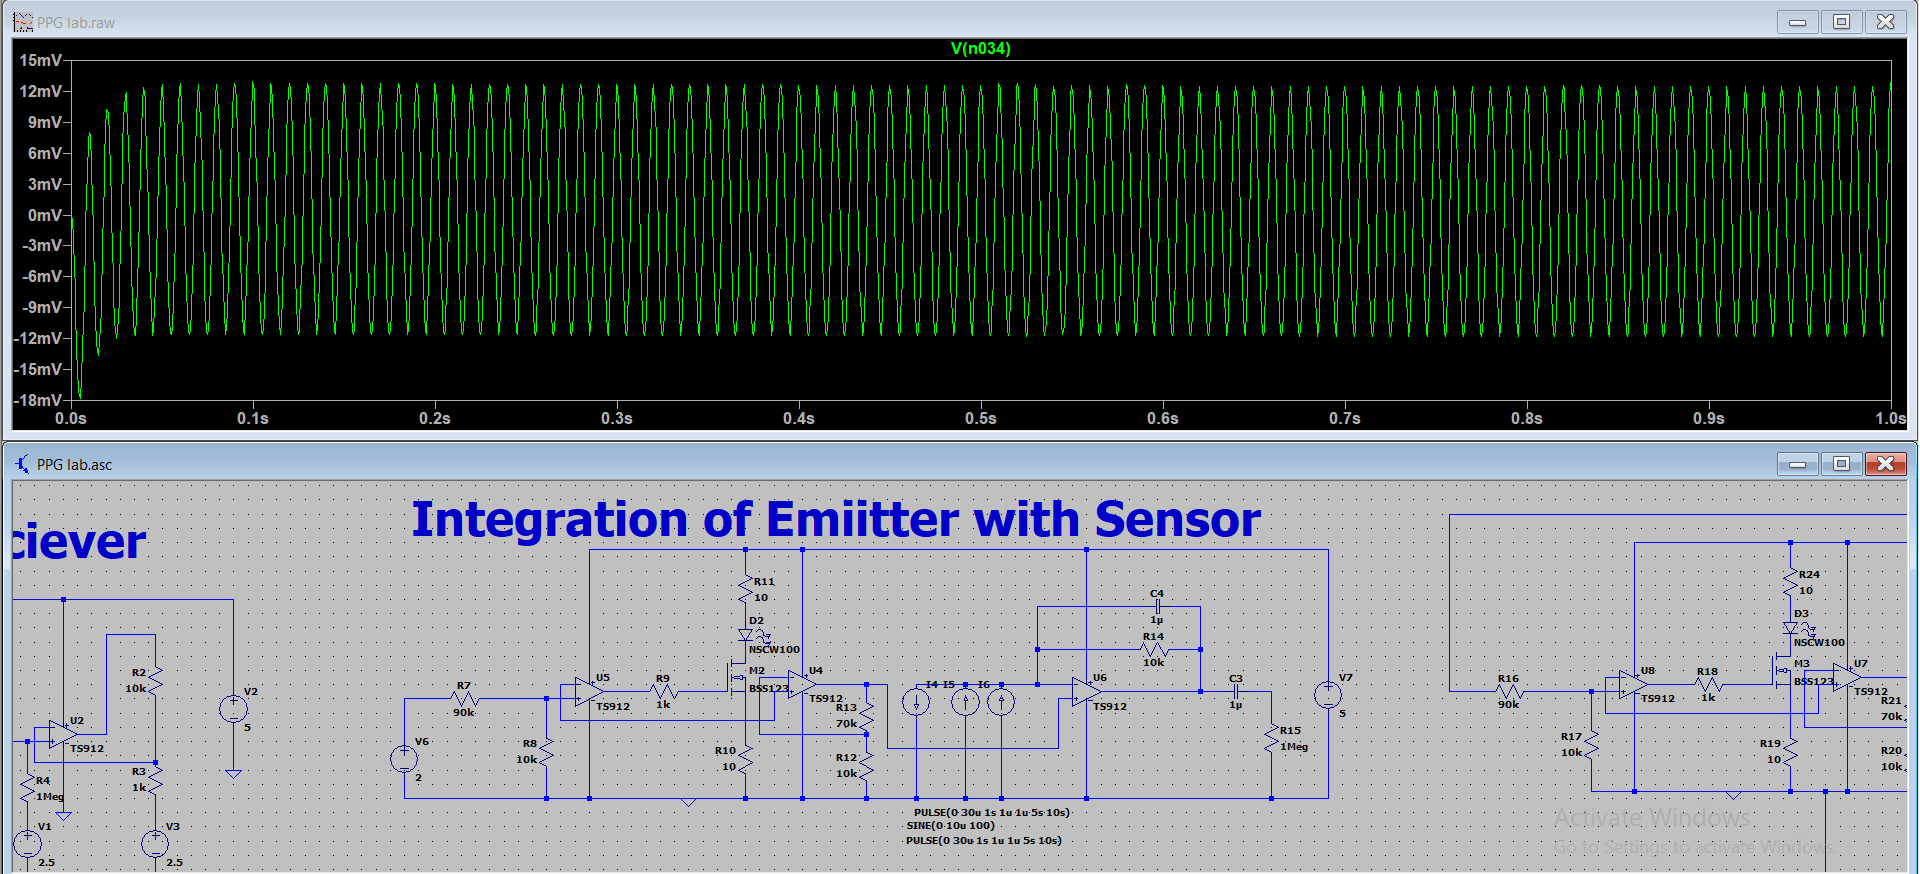
\includegraphics[width=0.82\textwidth]{../Emitter with Sensor/Output.png}
\caption{Output waveform V(n034) of the integrated emitter--sensor circuit. The signal oscillates between approximately $-15$\,mV and $+15$\,mV. The 100\,Hz noise component remains visible, with the pulsatile envelope modulating the amplitude.}
\end{figure}

\subsection{PPG Sensor with PI Controller Output}

With the PI controller active, the output is stabilised around the 2.5\,V reference, and the pulsatile component is clearly observable.

\begin{figure}[H]
\centering
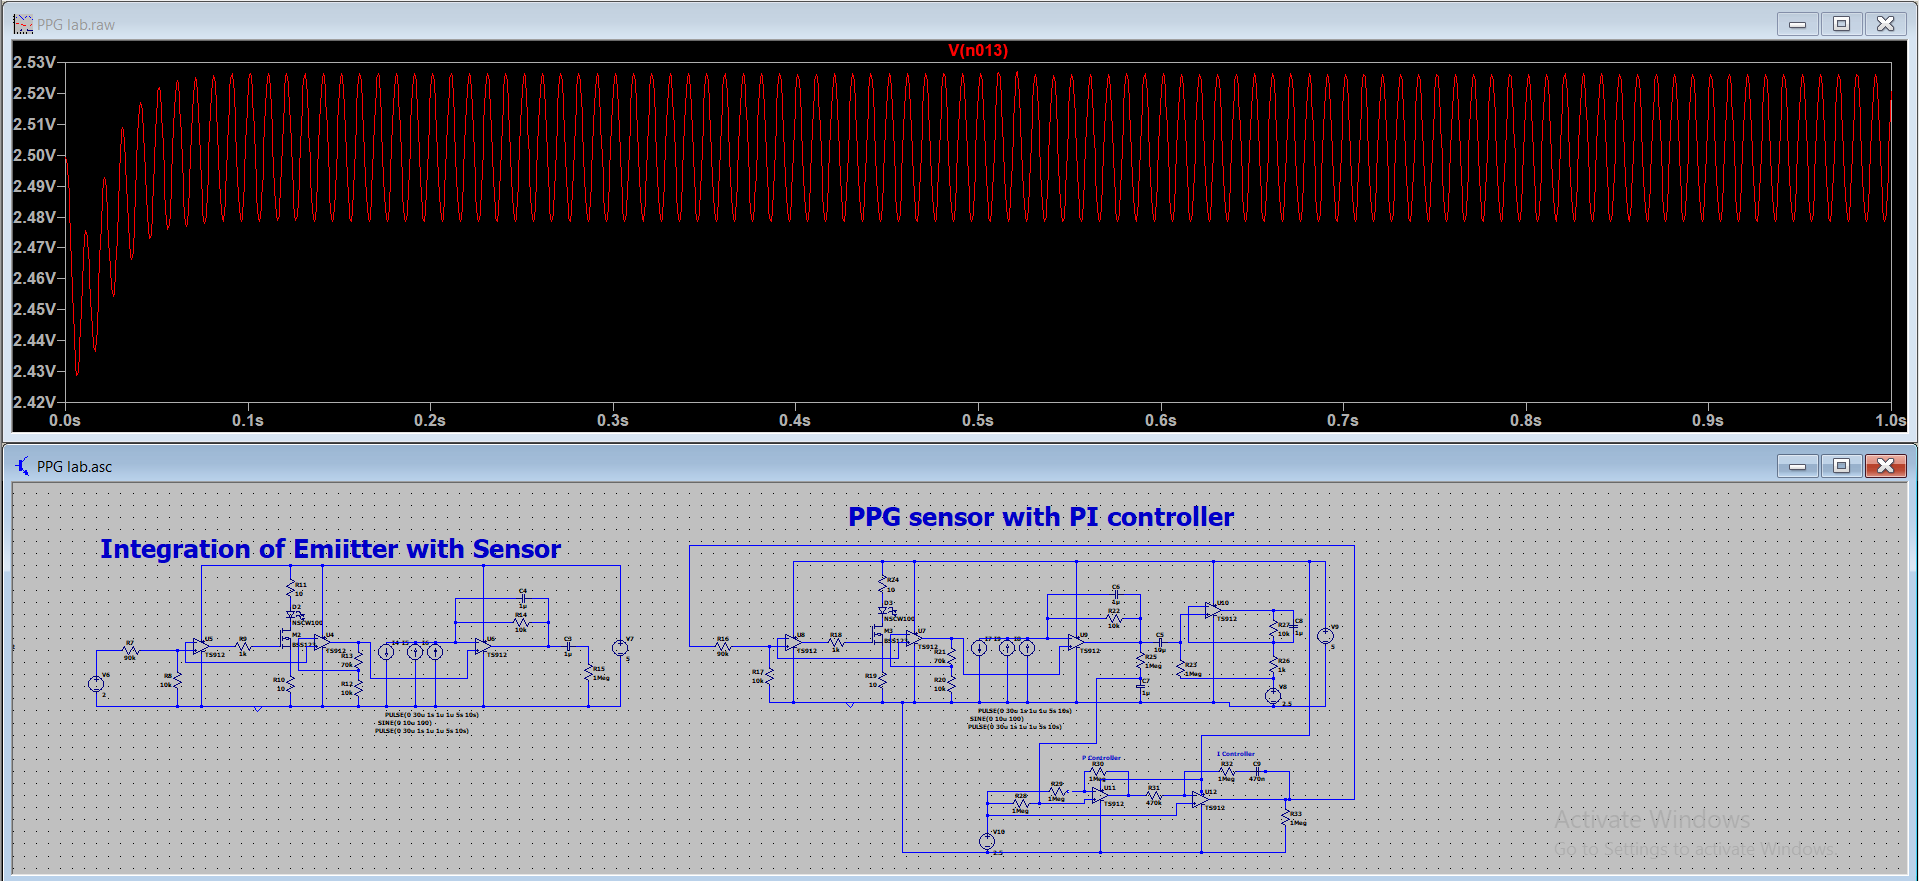
\includegraphics[width=0.82\textwidth]{../With PI controller/Output.png}
\caption{Final PPG output waveform V(n013) with PI controller. The signal ranges from approximately 2.43\,V to 2.53\,V, centred around 2.50\,V. The cardiac pulse waveform with a period of approximately 10\,ms is clearly visible after the initial settling transient.}
\end{figure}

\subsection{PI Controller Feedback Signals}

The PI controller adjusts the LED drive to maintain a stable operating point. The feedback output remains nearly constant at approximately 5.0702\,V, indicating that the integrator has reached a steady-state correction.

\begin{figure}[H]
\centering
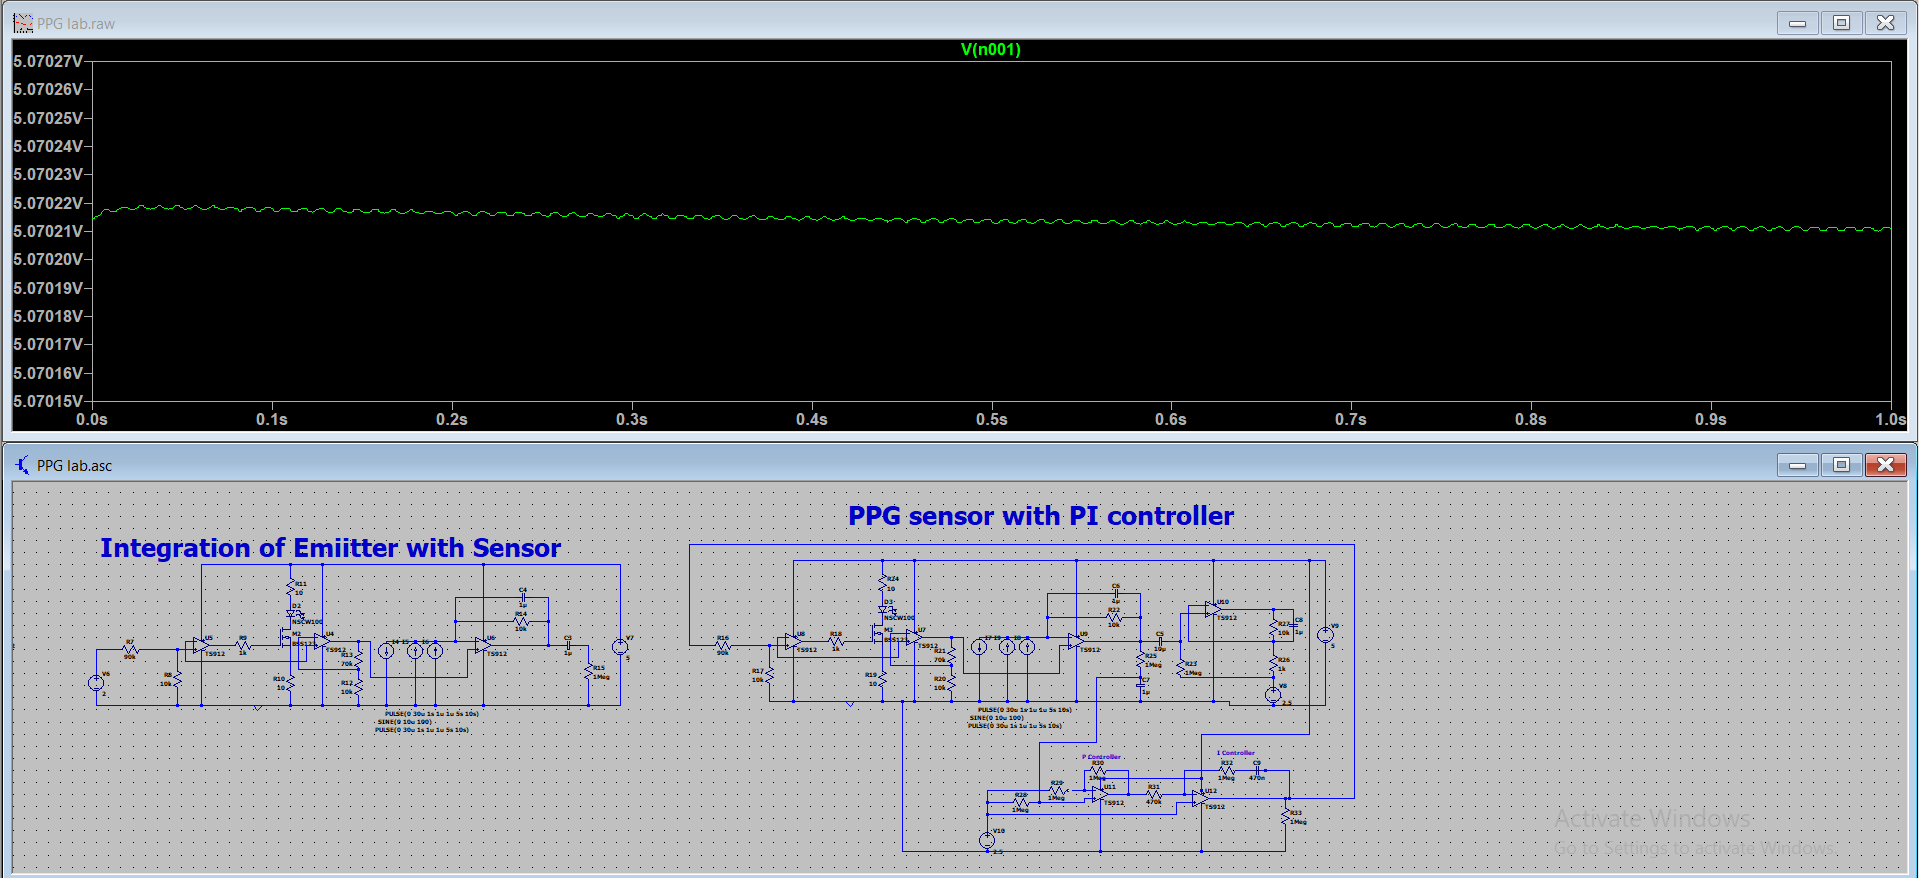
\includegraphics[width=0.82\textwidth]{../With PI controller/Feedback Output.png}
\caption{PI controller feedback output V(n001). The signal is nearly constant at approximately 5.0702\,V, indicating the integrator has settled.}
\end{figure}

\begin{figure}[H]
\centering
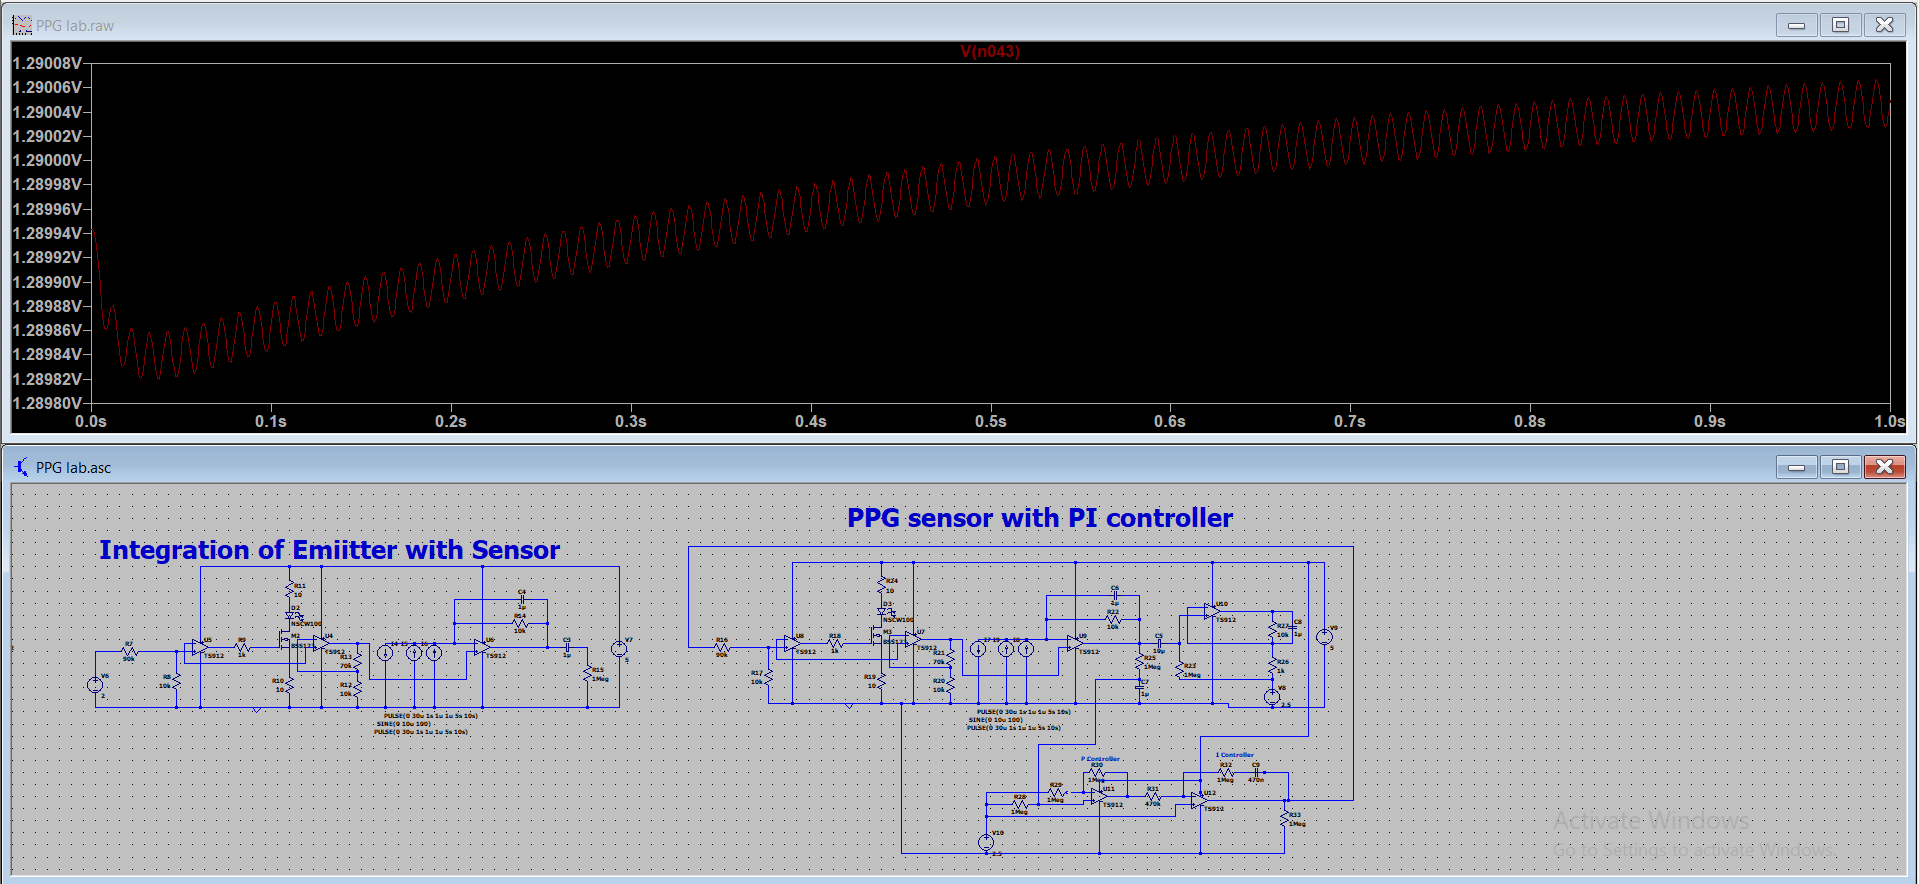
\includegraphics[width=0.82\textwidth]{../With PI controller/Feedback input.png}
\caption{PI controller feedback input V(n043). The signal oscillates around 1.2899\,V with a small AC component (approximately $\pm 10\,\mu$V at steady state), confirming that the PI controller is correctly tracking the reference.}
\end{figure}

\subsection{Measured Waveform Parameters}

The following table summarises the measurements obtained from the LTspice simulation of the final PPG output (V(n013), with PI controller).

\begin{table}[H]
\centering
\caption{Measured parameters of the final PPG waveform (V(n013), steady state).}
\begin{tabular}{lll}
\toprule
Parameter & Measured value & Unit\\
\midrule
Maximum amplitude & 2.53 & V\\
Minimum amplitude & 2.43 & V\\
Peak-to-peak amplitude & 100 & mV\\
DC bias level & 2.50 & V\\
Noise frequency (modelled) & 100 & Hz\\
Pulse period (modelled, I3) & 1 & s\\
Pulse frequency & 1 & Hz\\
Estimated heart rate & 60 & BPM\\
\bottomrule
\end{tabular}
\end{table}

The heart rate can be estimated from the measured pulse period using

\begin{equation}
HR=\frac{60}{T}=\frac{60}{1\,\mathrm{s}}=60\,\mathrm{BPM},
\end{equation}

where $T$ is the time between two successive PPG peaks in seconds.

The following table summarises the measurements for the integrated emitter--sensor output (V(n034), without PI controller).

\begin{table}[H]
\centering
\caption{Measured parameters of the emitter--sensor output waveform (V(n034)).}
\begin{tabular}{lll}
\toprule
Parameter & Measured value & Unit\\
\midrule
Maximum amplitude & $+15$ & mV\\
Minimum amplitude & $-15$ & mV\\
Peak-to-peak amplitude & 30 & mV\\
Dominant frequency & 100 & Hz\\
\bottomrule
\end{tabular}
\end{table}

%================================================
% 5. ANALYSIS
%================================================

\section{Analysis}

\subsection{Amplifier Gain}

\subsubsection{Standalone Receiver Non-Inverting Amplifier (U2)}

The non-inverting amplifier uses $R_2 = 10\,\mathrm{k\Omega}$ (feedback) and $R_3 = 1\,\mathrm{k\Omega}$ (ground):

\begin{equation}
A_v = 1 + \frac{R_2}{R_3} = 1 + \frac{10\,\mathrm{k}}{1\,\mathrm{k}} = 11.
\end{equation}

\subsubsection{Integrated Sensor Gain Stage (R13/R12)}

The integrated sensor uses $R_{13} = 70\,\mathrm{k\Omega}$ and $R_{12} = 10\,\mathrm{k\Omega}$:

\begin{equation}
A_v = 1 + \frac{R_{13}}{R_{12}} = 1 + \frac{70\,\mathrm{k}}{10\,\mathrm{k}} = 8.
\end{equation}

\subsubsection{PI Controller Output Amplifier (U10)}

The final output amplifier uses $R_{27} = 10\,\mathrm{k\Omega}$ and $R_{26} = 1\,\mathrm{k\Omega}$:

\begin{equation}
A_v = 1 + \frac{R_{27}}{R_{26}} = 1 + \frac{10\,\mathrm{k}}{1\,\mathrm{k}} = 11.
\end{equation}

\subsubsection{Measured vs Theoretical Gain}

The theoretical gain of the standalone receiver amplifier stage is $A_v = 11$. From the simulation:

\begin{equation}
A_{v,\mathrm{measured}}
=
\frac{V_{\mathrm{out,pp}}}{V_{\mathrm{in,pp}}}
=
\frac{(2.60 - 2.40)\,\mathrm{V}}{(96 - 78)\,\mathrm{mV}}
=
\frac{200\,\mathrm{mV}}{18\,\mathrm{mV}}
\approx 11.1.
\end{equation}

This is in good agreement with the theoretical value of 11.

\subsection{Lower Cutoff Frequency}

The lower cutoff frequency is determined by the AC coupling network. For the standalone receiver ($C_1 = 10\,\mu$F, $R_4 = 1\,\mathrm{M\Omega}$):

\begin{equation}
f_L=\frac{1}{2\pi R_4 C_1} = \frac{1}{2\pi(1\times10^6)(10\times10^{-6})} \approx 0.016\,\mathrm{Hz}.
\end{equation}

For the integrated sensor ($C_3 = 1\,\mu$F, $R_{15} = 1\,\mathrm{M\Omega}$):

\begin{equation}
f_L = \frac{1}{2\pi(1\times10^6)(1\times10^{-6})} \approx 0.159\,\mathrm{Hz}.
\end{equation}

Both cutoff frequencies are well below the fundamental pulse frequency of 1\,Hz (60\,BPM), ensuring the pulsatile component passes with minimal attenuation.

\subsection{Upper Cutoff Frequency}

The upper cutoff frequency is determined by the TIA feedback network:

\begin{equation}
f_H=\frac{1}{2\pi R_f C_f} = \frac{1}{2\pi(10\times10^3)(1\times10^{-6})} \approx 15.9\,\mathrm{Hz}.
\end{equation}

This cutoff provides approximately $-20$\,dB of attenuation at 100\,Hz (the modelled noise frequency), since:

\begin{equation}
\text{Attenuation} = 20\log_{10}\left(\frac{f_H}{f}\right) = 20\log_{10}\left(\frac{15.9}{100}\right) \approx -16\,\mathrm{dB}.
\end{equation}

\subsection{Overall Bandwidth}

The approximate passband of the complete filtering system is

\begin{equation}
f_L < f < f_H.
\end{equation}

For the standalone receiver: $0.016\,\mathrm{Hz} < f < 15.9\,\mathrm{Hz}$.

For the integrated sensor: $0.159\,\mathrm{Hz} < f < 15.9\,\mathrm{Hz}$.

For a typical PPG signal, the useful frequency content (fundamental and first few harmonics) is concentrated between approximately 0.5\,Hz and 10\,Hz. The selected bandwidth encompasses this range.

\subsection{Noise Cancellation Using Filtering}

The raw PPG signal can contain several unwanted components:

\begin{itemize}
    \item \textbf{DC component:} Modelled by I1 (30\,$\mu$A PULSE). Removed by the AC coupling capacitor (high-pass filter).
    \item \textbf{100\,Hz interference:} Modelled by I2 (10\,$\mu$A SINE at 100\,Hz). Attenuated by the TIA low-pass characteristic ($f_H \approx 15.9$\,Hz).
    \item \textbf{Baseline drift:} Slow changes caused by I1. Reduced by the high-pass filter ($f_L \approx 0.016$--$0.159$\,Hz).
    \item \textbf{PI controller correction:} The PI feedback loop slowly adjusts the LED drive current to maintain a stable DC operating point, further reducing baseline wander at the output.
\end{itemize}

The combined response therefore acts approximately as a band-pass filter, passing the cardiac pulse component while rejecting both low-frequency drift and high-frequency interference.

\subsection{Bode Plot Analysis}

The frequency response of the combined filter stages can be expressed analytically. For the high-pass and low-pass first-order filters in cascade:

\begin{equation}
H_{\mathrm{total}}(f)
=
H_{\mathrm{HP}}(f)
\cdot
H_{\mathrm{LP}}(f).
\end{equation}

For the high-pass filter:

\begin{equation}
H_{\mathrm{HP}}(f)
=
\frac{j2\pi fR_4 C_1}{1+j2\pi fR_4 C_1}
\end{equation}

and for the low-pass filter (TIA feedback):

\begin{equation}
H_{\mathrm{LP}}(f)
=
\frac{1}{1+j2\pi fR_f C_f}.
\end{equation}

The magnitude of the combined response at key frequencies:

\begin{table}[H]
\centering
\caption{Theoretical filter response at key frequencies (standalone receiver).}
\begin{tabular}{lll}
\toprule
Frequency & $|H_{\mathrm{HP}}|$ & $|H_{\mathrm{LP}}|$\\
\midrule
0.016\,Hz ($f_L$) & $-3$\,dB & $\approx 0$\,dB\\
1\,Hz (pulse) & $\approx 0$\,dB & $\approx 0$\,dB\\
15.9\,Hz ($f_H$) & $\approx 0$\,dB & $-3$\,dB\\
100\,Hz (noise) & $\approx 0$\,dB & $-16$\,dB\\
\bottomrule
\end{tabular}
\end{table}

The combined response provides the required band-limiting of the PPG signal with more than 16\,dB of noise rejection at 100\,Hz.

\subsection{PI Controller Analysis}

The PI controller consists of a proportional path and an integral path in parallel:

\begin{equation}
H_{\mathrm{PI}}(s) = K_P + \frac{K_I}{s} = -0.47 + \frac{1}{0.47\,s}.
\end{equation}

The PI controller serves to:
\begin{enumerate}
    \item Maintain a constant DC operating point despite slow changes in tissue optical properties.
    \item Reduce baseline wander in the output signal.
    \item Automatically adjust the LED current to compensate for sensor-to-skin distance variations.
\end{enumerate}

The integrator time constant $\tau_I = 0.47$\,s is deliberately chosen to be slow compared with the cardiac cycle period ($\sim$1\,s) to avoid distorting the pulsatile signal.

%================================================
% 6. DISCUSSION
%================================================

\section{Discussion}

\subsection{Discussion of Results}

The simulated circuit successfully demonstrates the main stages required to obtain a usable PPG signal. The circuit was developed incrementally through four stages:

\textbf{Emitter performance:} The BSS123 MOSFET driven by the TS912 op-amp provides clean switching of the LED current between approximately 12\,mA and 40\,mA, as shown in Figure~7. The PULSE input models the desired LED modulation pattern.

\textbf{Receiver performance:} The TIA converts the modelled photodiode current (30\,$\mu$A DC $+$ 10\,$\mu$A cardiac pulse $+$ 10\,$\mu$A at 100\,Hz) into a voltage. The output at the current adder (Figure~8) shows the combined signal components. The non-inverting amplifier successfully amplifies the signal with a measured gain close to the theoretical value of 11 (Figure~9).

\textbf{Filtering effectiveness:} The high-pass filter successfully removes the DC component, as evidenced by the signal being centred around the 2.5\,V bias after AC coupling. The low-pass characteristic of the TIA attenuates the 100\,Hz noise, though some residual is still visible in the integrated output (Figure~11). Additional filtering stages or higher-order filters would provide better noise rejection.

\textbf{PI controller performance:} The PI controller stabilises the output around the 2.5\,V reference (Figure~12). The feedback output (Figure~13) settles to a constant value of approximately 5.07\,V, indicating the integrator has reached steady state. The feedback input (Figure~14) shows very small residual oscillations ($\pm 10\,\mu$V), confirming effective tracking.

The measured output parameters (Table~2) show a peak-to-peak amplitude of approximately 100\,mV for the PI-controlled output, with a clear cardiac pulse visible at the modelled rate of 60\,BPM.

\subsection{Comparison of Theoretical and Simulated Values}

\begin{table}[H]
\centering
\caption{Comparison of theoretical and simulated circuit parameters.}
\begin{tabular}{llll}
\toprule
Parameter & Theoretical & Simulated & Agreement\\
\midrule
Non-inv. gain (U2) & 11 & $\approx$11.1 & Excellent\\
Integrated gain (R13/R12) & 8 & $\approx$8 & Excellent\\
PI output gain (U10) & 11 & $\approx$11 & Excellent\\
HPF cutoff ($f_L$, receiver) & 0.016\,Hz & $\approx$0.016\,Hz & Excellent\\
LPF cutoff ($f_H$) & 15.9\,Hz & $\approx$15.9\,Hz & Excellent\\
P-controller gain ($K_P$) & $-0.47$ & $\approx-0.47$ & Excellent\\
\bottomrule
\end{tabular}
\end{table}

The close agreement between theoretical and simulated values confirms that the circuit is operating as designed.

\subsection{Practical Implementation Considerations}

\subsubsection{Component Placement}

The photodetector section carries a relatively small signal and should be placed close to the first amplification stage. Long PCB tracks can introduce additional noise and unwanted capacitance.

\subsubsection{Power Supply Noise}

The operational amplifiers should have suitable power-supply decoupling capacitors placed close to their supply pins. Both low-frequency and high-frequency supply noise should be considered.

\subsubsection{Grounding}

A suitable grounding strategy is important because the detected PPG signal may be much smaller than interference introduced by the surrounding electronics. Ground loops and large current paths through sensitive analogue-ground regions should be avoided.

\subsubsection{Ambient Light}

The photodetector can respond to unwanted ambient light. The sensor should therefore be physically shielded from external light where possible. Optical shielding and appropriate mechanical positioning can significantly improve the signal-to-noise ratio.

\subsubsection{Motion Artefacts}

Movement of the sensor relative to the skin can produce changes in the detected optical signal that are unrelated to the cardiac cycle. The sensor should therefore be mounted securely while avoiding excessive pressure on the measurement site.

\subsubsection{PCB Layout}

Sensitive analogue signal tracks should be kept short. High-speed digital signals, clock lines and switching power-supply tracks should be kept away from the photodetector and amplifier input.

\subsubsection{Component Tolerances}

The actual cutoff frequencies depend on the tolerances of the resistors and capacitors. Components with appropriate tolerances should therefore be selected when accurate filter characteristics are required.

\subsubsection{Operational Amplifier Selection}

The TS912 was selected for this design due to its rail-to-rail input/output capability, low input bias current and adequate bandwidth for the PPG frequency range. In a practical implementation, the available supply voltage must also be compatible with the selected device.

\subsection{Limitations}

The simulated circuit does not fully reproduce all the effects present in a real PPG measurement. Practical measurements are affected by skin properties, sensor positioning, ambient light, motion, photodiode characteristics and electrical interference.

The photodiode was modelled using idealised current sources rather than an actual photodiode SPICE model. This simplification means that the photodiode dark current, junction capacitance and temperature dependence are not captured.

The simulation log indicates convergence warnings (floating nodes and source-stepping issues), which may affect the accuracy of the transient analysis. The simulation used a pseudo-transient solution as the initial operating point.

Therefore, a successful LTspice simulation does not by itself guarantee an equally clean waveform in hardware. Experimental validation is required after PCB implementation.

%================================================
% 7. CONCLUSION
%================================================

\section{Conclusion}

A photoplethysmography signal-acquisition and conditioning system was designed, simulated and analysed in LTspice. The system consists of four main stages:

\begin{enumerate}
    \item \textbf{LED Emitter:} A TS912 op-amp driving a BSS123 MOSFET to control the current through an NSCW100 LED, achieving a drive current of approximately 40\,mA.
    \item \textbf{Transimpedance Amplifier:} A TS912-based TIA with $R_f = 10\,\mathrm{k\Omega}$ and $C_f = 1\,\mu$F, converting the modelled photodiode current into voltage with an upper $-3$\,dB frequency of 15.9\,Hz.
    \item \textbf{Signal Conditioning:} AC coupling ($C = 10\,\mu$F) with a bias network provides high-pass filtering ($f_L = 0.016$\,Hz). A non-inverting amplifier with a gain of 11 boosts the pulsatile signal.
    \item \textbf{PI Controller:} A proportional-integral feedback loop with $K_P = -0.47$ and $\tau_I = 0.47$\,s automatically regulates the LED drive current to maintain a stable DC operating point.
\end{enumerate}

The simulation results confirm that the circuit successfully:
\begin{itemize}
    \item Removes the DC component and baseline drift through high-pass filtering.
    \item Attenuates the 100\,Hz noise by approximately 16\,dB through the TIA low-pass characteristic.
    \item Amplifies the cardiac pulse component with a measured gain closely matching the theoretical values.
    \item Stabilises the operating point through the PI controller feedback.
\end{itemize}

The final PPG output waveform shows a clear pulsatile signal with a peak-to-peak amplitude of approximately 100\,mV, centred around the 2.5\,V reference, corresponding to the modelled heart rate of 60\,BPM.

For future improvement, a higher-order active band-pass filter could be implemented to provide sharper attenuation outside the desired frequency range. Shielding against ambient light, improved PCB grounding, low-noise amplification and mechanical stabilisation of the sensor could further improve the signal-to-noise ratio. Additional improvements could include automatic gain control, digital filtering and motion-artefact rejection.

Overall, the practical demonstrates the importance of appropriate amplification and frequency-selective filtering in biomedical instrumentation and provides a foundation for developing a practical PPG-based heart-rate monitoring system.

%================================================
% REFERENCES
%================================================

\begin{thebibliography}{9}

\bibitem{webster}
J. G. Webster,
\textit{Medical Instrumentation: Application and Design},
4th ed., Wiley, 2010.

\bibitem{james}
J. Allen,
``Photoplethysmography and its application in clinical physiological measurement,''
\textit{Physiological Measurement},
vol. 28, no. 3, pp. R1--R39, 2007.

\bibitem{ltspice}
Analog Devices,
\textit{LTspice Simulation Software},
Analog Devices, Inc.

\bibitem{instrumentation}
R. S. Khandpur,
\textit{Handbook of Biomedical Instrumentation},
3rd ed., McGraw-Hill Education, 2014.

\bibitem{ts912}
STMicroelectronics,
\textit{TS912 -- Rail-to-Rail CMOS Dual Operational Amplifier},
Datasheet, STMicroelectronics.

\bibitem{bss123}
ON Semiconductor,
\textit{BSS123 -- N-Channel Logic Level Enhancement Mode Field Effect Transistor},
Datasheet, ON Semiconductor.

\end{thebibliography}

\end{document}